\begin{figure}[H]
    \centering
    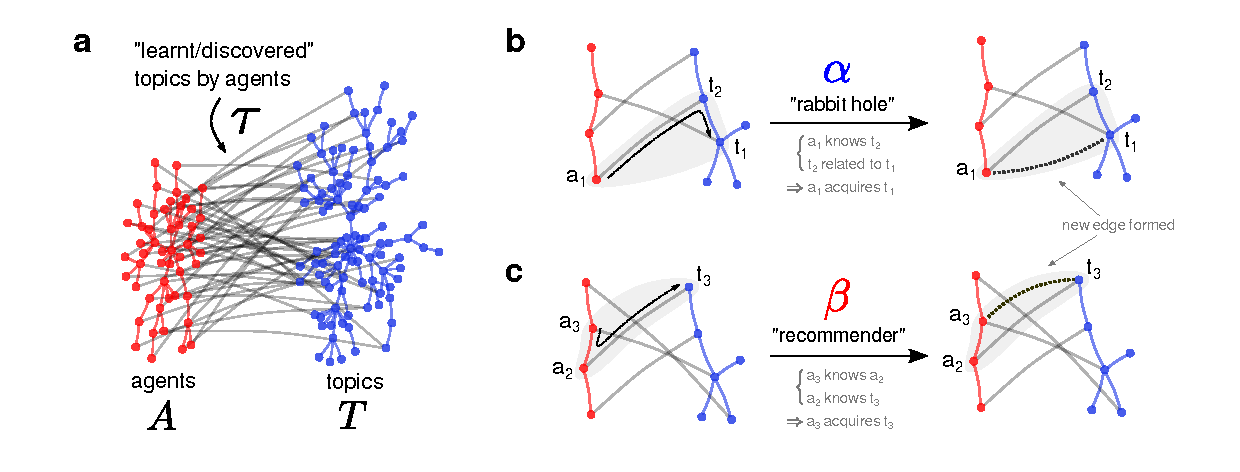
\includegraphics[width=0.95\textwidth,center]{../figures/report/Fig1.pdf}
    \caption{\label{fig:1}
    \textit{Model setup and description of the update process}.
    (\textbf{a}) Illustration of the intralayer agent graph (red) and topic graph (blue) with the interlayer edges (gray) representing the knowledge set of the agents.
    (\textbf{b}) and (\textbf{c}) illustrate the update process either through learning/discovery by related topics ("rabbit-hole") or learning/discovery through friends ("recommender")
    }
\end{figure}